\documentclass[notes,11pt, aspectratio=169]{beamer}

\usepackage{pgfpages}
% These slides also contain speaker notes. You can print just the slides,
% just the notes, or both, depending on the setting below. Comment out the want
% you want.
\setbeameroption{hide notes} % Only slide
%\setbeameroption{show only notes} % Only notes
%\setbeameroption{show notes on second screen=right} % Both

%\usepackage[scaled=1.0]{helvet}
\usepackage{array}


\usepackage{tikz}
\usepackage{verbatim}
\setbeamertemplate{note page}{\pagecolor{gray!5}\insertnote}
\usetikzlibrary{positioning}
\usetikzlibrary{snakes}
\usetikzlibrary{calc}
\usetikzlibrary{arrows}
\usetikzlibrary{decorations.markings}
\usetikzlibrary{shapes.misc}
\usetikzlibrary{matrix,shapes,arrows,fit,tikzmark}
\usepackage{amsmath}
\usepackage{mathpazo}
\usepackage{hyperref}
\usepackage{lipsum}
\usepackage{multimedia}
\usepackage{graphicx}
\usepackage{multirow}
\usepackage{graphicx}
\usepackage{dcolumn}
\usepackage{bbm}
\newcolumntype{d}[0]{D{.}{.}{5}}

\usepackage{changepage}
\usepackage{appendixnumberbeamer}
\newcommand{\beginbackup}{
   \newcounter{framenumbervorappendix}
   \setcounter{framenumbervorappendix}{\value{framenumber}}
   \setbeamertemplate{footline}
   {
     \leavevmode%
     \hline
     box{%
       \begin{beamercolorbox}[wd=\paperwidth,ht=2.25ex,dp=1ex,right]{footlinecolor}%
%         \insertframenumber  \hspace*{2ex} 
       \end{beamercolorbox}}%
     \vskip0pt%
   }
 }
\newcommand{\backupend}{
   \addtocounter{framenumbervorappendix}{-\value{framenumber}}
   \addtocounter{framenumber}{\value{framenumbervorappendix}} 
}


\usepackage{graphicx}
\usepackage[space]{grffile}
\usepackage{booktabs}

% These are my colors -- there are many like them, but these ones are mine.
\definecolor{blue}{RGB}{0,114,178}
\definecolor{red}{RGB}{213,94,0}
\definecolor{yellow}{RGB}{240,228,66}
\definecolor{green}{RGB}{0,158,115}

\hypersetup{
  colorlinks=false,
  linkbordercolor = {white},
  linkcolor = {blue}
}


%% I use a beige off white for my background
\definecolor{MyBackground}{RGB}{255,253,218}

%% Uncomment this if you want to change the background color to something else
%\setbeamercolor{background canvas}{bg=MyBackground}

%% Change the bg color to adjust your transition slide background color!
\newenvironment{transitionframe}{
  \setbeamercolor{background canvas}{bg=white}
  \begin{frame}}{
    \end{frame}
}

\setbeamercolor{frametitle}{fg=blue}
\setbeamercolor{title}{fg=black}
\setbeamertemplate{footline}[frame number]
\setbeamertemplate{navigation symbols}{} 
\setbeamertemplate{itemize items}{-}
\setbeamercolor{itemize item}{fg=blue}
\setbeamercolor{itemize subitem}{fg=blue}
\setbeamercolor{enumerate item}{fg=blue}
\setbeamercolor{enumerate subitem}{fg=blue}
\setbeamercolor{button}{bg=MyBackground,fg=blue,}

%%% TIKZ STUFF
\tikzset{   
	every picture/.style={remember picture,baseline},
	every node/.style={anchor=base,align=center,outer sep=1.5pt},
	every path/.style={thick},
}
\newcommand\marktopleft[1]{%
	\tikz[overlay,remember picture] 
	\node (marker-#1-a) at (-.3em,.3em) {};%
}
\newcommand\markbottomright[2]{%
	\tikz[overlay,remember picture] 
	\node (marker-#1-b) at (0em,0em) {};%
}
\tikzstyle{every picture}+=[remember picture] 
\tikzstyle{mybox} =[draw=black, very thick, rectangle, inner sep=10pt, inner ysep=20pt]
\tikzstyle{fancytitle} =[draw=black,fill=red, text=white]
%%%% END TIKZ STUFF


% If you like road maps, rather than having clutter at the top, have a roadmap show up at the end of each section 
% (and after your introduction)
% Uncomment this is if you want the roadmap!
% \AtBeginSection[]
% {
%    \begin{frame}
%        \frametitle{Roadmap of Talk}
%        \tableofcontents[currentsection]
%    \end{frame}
% }
\setbeamercolor{section in toc}{fg=blue}
\setbeamercolor{subsection in toc}{fg=red}
\setbeamersize{text margin left=1em,text margin right=1em} 

\newenvironment{wideitemize}{\itemize\addtolength{\itemsep}{10pt}}{\enditemize}
\newenvironment{wideenumerate}{\enumerate\addtolength{\itemsep}{10pt}}{\endenumerate}

\usepackage{environ}
\NewEnviron{videoframe}[1]{
  \begin{frame}
    \vspace{-8pt}
    \begin{columns}[onlytextwidth, T] % align columns
      \begin{column}{.58\textwidth}
        \begin{minipage}[t][\textheight][t]
          {\dimexpr\textwidth}
          \vspace{8pt}
          \hspace{4pt} {\Large \sc \textcolor{blue}{#1}}
          \vspace{8pt}
          
          \BODY
        \end{minipage}
      \end{column}%
      \hfill%
      \begin{column}{.42\textwidth}
        \colorbox{green!20}{\begin{minipage}[t][1.2\textheight][t]
            {\dimexpr\textwidth}
            Face goes here
          \end{minipage}}
      \end{column}%
    \end{columns}
  \end{frame}
}

\title[]{\textcolor{blue}{ECN 453: Pricing and Price Discrimination 1}}
\author[PGP]{}
\institute[FRBNY]{\small{\begin{tabular}{c c c}
Nicholas Vreugdenhil \\
\end{tabular}}}
\date{} 

\begin{document}

% Title Slide
\begin{frame}
\maketitle
  \centering
\end{frame}

% INTRO

\begin{frame}{Price Discrimination}
\begin{wideitemize}
	\item Price discrimination: \textbf{setting different prices for the same good}.
	\item Examples: airline tickets, software, pharmaceuticals
	\vspace{-10pt}
	\begin{figure}
	\item \includegraphics[scale=0.13]{airline.jpeg}
	\caption{Photo: Flickr}
	\end{figure}
	\item We will look at different ways that firms price discriminate and the implications for policy.
	%\item One surprising outcome we will discuss is that sometimes price discrimination can make consumers better off (!)
\end{wideitemize}
\end{frame}

\begin{frame}{Plan}
  \begin{wideenumerate}
  	\item Why price discriminate?
  	\item Price discrimination: selection by indicators
  \end{wideenumerate}
\end{frame}

\begin{frame}{Plan}
	\begin{wideenumerate}
		\item \textbf{Why price discriminate?}
		\item Price discrimination: selection by indicators
	\end{wideenumerate}
\end{frame}

\begin{frame}{Why price discriminate?}
		\begin{wideitemize}
			\item Previously, we studied a monopolist who could only set \textbf{one price}.
			\item In the following diagram, I argue that a monopolist could increase profit if it could set \textbf{different prices for different consumers}.
		\end{wideitemize}
\end{frame}

\begin{frame}{Why price discriminate?: Monopoly diagram}
	\begin{figure}
		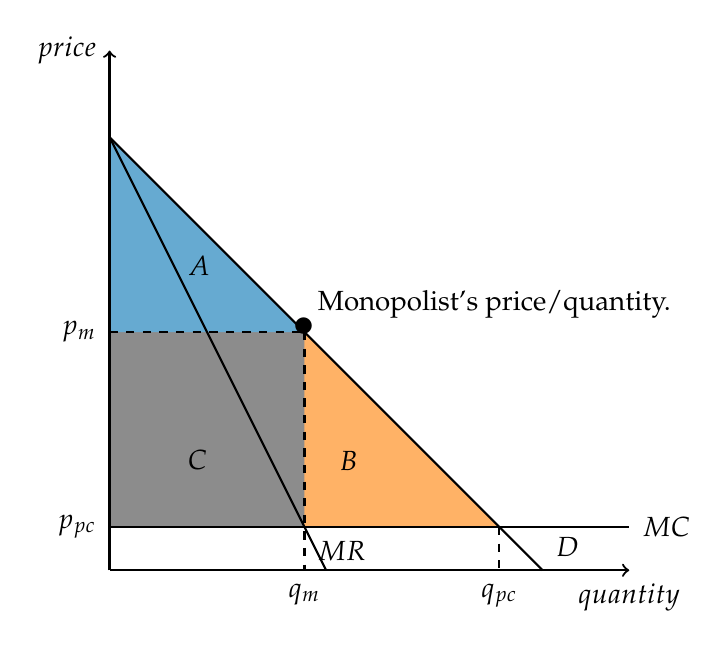
\begin{tikzpicture}[scale=0.55]
			\fill [darkgray!60] (0,1) -- (0,5.5) -- (4.5,5.5) -- (5.5,1) -- cycle;
			\fill [blue!60] (0,5.5) -- (4.5,5.5) -- (0,10) -- cycle;
			\fill [orange!60] (4.5,1) -- (4.5,5.5) -- (9,1) -- cycle;
			
			%y axis.....................
			\draw [->] (0,0) to (0,12) node [left] {$price$};
			
			%x axis......................
			\draw [->] (0,0) to (12,0) node [below] {$quantity$};
			
			% D curve...................
			\draw [thick] (0,10)  to  (10,0)  node [above right] {$D$};
			
			% MR curve....................
			\draw [thick] (0,10) to (5,0);
			\node [above right] at (4.5,-0.1) {$MR$};
			
			% MC=S curve...................
			\draw [thick] (0,1)  to  (12,1)  node [right] {$MC$};
			
			% dashed lines to equilibrium.............
			\draw [dashed] (0,5.5) node [left] {$p_m$} to (4.55,5.5); 
			\draw [dashed] (4.5,5.5) to (4.5,0) node [below] {$q_m$};
			
			% dashed lines to new equilibrium.........
			\draw [dashed] (0,1) node [left] {$p_{pc}$} to (9,1); 
			\draw [dashed] (9,1) to (9,0) node [below] {$q_{pc}$};
			
			% equilibrium points.......................
			\node [black] at (4.5,5.25) {\LARGE \textbullet};
			
			% labels..............................
			\node [black, above right] at (4.5,5.5) {Monopolist's price/quantity.};
			\node [above right] at (1.5,6.5) {$A$};
			\node [above right] at (5,2) {$B$};
			\node [above right] at (1.5,2) {$C$};
		\end{tikzpicture}
	\end{figure}
\end{frame}

\begin{frame}{Why price discriminate?: Monopoly diagram}
	\begin{wideitemize}
		\item On the previous slide there are three areas:
		\vspace{11pt}
	\end{wideitemize}
	\begin{wideenumerate}
		\item \textbf{Area A}: consumers who are willing to pay a price higher than $p_m$. 
			\begin{wideitemize}
				\item This was consumer surplus (when monopolist can only set one price)
				\item Monopolist could increase profits if it set \underline{higher prices} for these consumers.
			\end{wideitemize}
		\item \textbf{Area B}: consumers who are willing to pay a price lower than $p_m$, but higher than MC. 
			\begin{wideitemize}
				\item This was dead-weight-loss (when the monopolist can only set one price)
				\item The monopolist could increase profits if it set \underline{lower prices} for these consumers and sold to them.
			\end{wideitemize}
		\item \textbf{Area C}: this is the current profit of the monopolist.
	\end{wideenumerate}
\end{frame}

\begin{frame}{Why price discriminate?: Monopoly diagram}
		\begin{wideitemize}
			\item In order to fully extract all of area $A$ and $B$ in the previous diagram, the monopolist would have to know the \underline{exact willingness to pay} of each consumer in the market.
			\item This is called \textbf{perfect price discrimination}.
						\begin{wideitemize}
							\item Specifically, the monopolist charges each consumer a price equal to their exact willingness to pay.
							\item It is also known as `first-degree price discrimination'.
						\end{wideitemize}
			\item Perfect price discrimination is a useful - but unrealistic - benchmark
			\item In practice, firms only have limited information about each consumer's willingness to pay. 
			\begin{wideitemize}
				\item We will now see some alternative forms of price discrimination when firms have more limited information about consumers.
			\end{wideitemize}
		\end{wideitemize}
\end{frame}

\begin{frame}{Plan}
	\begin{wideenumerate}
		\item Why price discriminate?
		\item \textbf{Price discrimination: selection by indicators}
	\end{wideenumerate}
\end{frame}

\begin{frame}{Price discrimination: selection by indicators}
	\begin{wideitemize}
		\item \textbf{Selection by indicators} is when the seller divides buyers into groups, setting a different price for each group.
		\item \textbf{Example:} Car sales
	\end{wideitemize}
	\begin{columns}[onlytextwidth, T] 
	\begin{column}{.5\textwidth}
		\begin{figure}
			\begin{tabular}{|c|c|c|}
				\hline
				Model & Italy & UK  \\
				\hline
				Fiat Uno& 21.7  & 8.7  \\
				Nissan Micra& 36.1  & 12.5  \\
				Mercedes 190 & 15.6  & 12.3  \\
				\hline
			\end{tabular}
			\caption{Car margins across countries}
		\end{figure}
	\end{column}
	\begin{column}{.5\textwidth}
				\begin{figure}
					\includegraphics[scale=0.12]{rav4.png}
				\end{figure}
			\end{column}
	\end{columns}
\end{frame}

\begin{frame}{Price discrimination: selection by indicators}
	\begin{wideitemize}
		\item Selection by indicators requires the buyer to have information about which groups consumers belong to.
		\item Other examples:
		\begin{wideitemize}
			\vspace{11pt}
			\item Movie tickets (students vs non-students)
			\item Other forms of geographical price discrimination (pharmaceuticals in developing vs non-developing countries)
			\item Different prices due to differences in browsing history/cookies on the internet
		\end{wideitemize}
		\item Selection by indicators is also known as `third-degree price discrimination'.
	\end{wideitemize}
\end{frame}

\begin{frame}{Price discrimination: selection by indicators}
\begin{wideitemize}
	\item \textbf{Setup}:
	\item Two markets denoted 1 and 2.
	\item \underline{Demand}:
	\begin{wideitemize}
		\item market 1: $q_1=D_1(p_1)$ 
		\item market 2: $q_2=D_2(p_2)$
	\end{wideitemize}
	\item \underline{Total cost}: $C(Q)$ where the total quantity $Q$ is:
	 \begin{align*}
	 	Q=q_1 + q_2 =D_1(p_1) + D_2(p_2)
	\end{align*}
	%\item \underline{Total profit} $\Pi(p_1,p_2)$ is given by:
	%\begin{align*}
	%	\Pi(p_1,p_2) = p_1 D_1(p1) + p_2 D_2(p_2) - C(D_1(p1) + D_2(p_2))
	%\end{align*}
	\item \textbf{Aim:} Find the optimal price (the profit maximizing price) in each market.
\end{wideitemize}
\end{frame}

\begin{frame}{Price discrimination: selection by indicators}
	\begin{wideitemize}
		\item \textbf{Solution}: Idea - \textbf{``optimal pricing rule in each market''}
		%\begin{wideitemize}
		%	\item This is the intuition with a constant marginal cost. Things get a little more complicated with a non-constant marginal cost, but we will ignore these situations in this course.
		%\end{wideitemize}
		\item \underline{Method 1:} The optimal price is where:
		\begin{align*}
			MR_1 = MC \text{ and } MR_2 = MC 
		\end{align*}
		\item In the above equation, $MR_1$ is marginal revenue in market 1, $MR_2$ is marginal revenue in market 2
		\item  \underline{Method 2:} Optimal prices must satisfy the elasticity rule:
		\begin{align*}
			p_1 (1+\frac{1}{\epsilon_1}) = MC \text{ and } 	p_2 (1+\frac{1}{\epsilon_2}) = MC
		\end{align*}
		\item In the above equation, $\epsilon_1$ and $\epsilon_2$ are the price elasticities of demand.
		%\item *(Optional math proving these results on the next slide, or you can just remember and apply the above results.)
	\end{wideitemize}
\end{frame}

\begin{frame}{Price discrimination: selection by indicators}
	\begin{wideitemize}
		\item Implication of optimal pricing under discrimination by market segmentation:
		\vspace{11pt}
		\begin{center}
			\textit{A seller should charge a higher price in those market segments with more inelastic demand.}
		\end{center}
		\item \textbf{Why?} Dividing the two optimal prices in terms of the elasticity rule:
	\begin{align*}
		\frac{p_1}{p_2} =  \frac{(1+\frac{1}{\epsilon_2})}{(1+\frac{1}{\epsilon_1})}
	\end{align*}
		\item Since demand elasticities are negative, the elasticity in market 1 is more inelastic than market 2 if $\epsilon_1 > \epsilon_2$.
		\item If $\epsilon_1 > \epsilon_2$, then $1+\frac{1}{\epsilon_2} > 1+\frac{1}{\epsilon_1}$ and so $ \frac{(1+\frac{1}{\epsilon_2})}{(1+\frac{1}{\epsilon_1})} > 1$
		\item Using the above equation implies that $p_1 > p_2$.
	\end{wideitemize}	
\end{frame}

\begin{frame}{Price discrimination: selection by indicators}
	\begin{wideitemize}
		\item Implication of optimal pricing under discrimination by market segmentation:
		\vspace{11pt}
		\begin{center}
			\textit{A seller should charge a higher price in those market segments with more inelastic demand.}
		\end{center}
		\item Note: this statement can be a little confusing when you come to apply it because demand price elasticity is negative
		\begin{wideitemize}
			\item Just remember that `more inelastic' means lower absolute values so that e.g. a market with $\epsilon=-2$ is more inelastic than a market with $\epsilon=-4$
		\end{wideitemize}
		\item We will now see particular example of the above statement.
	\end{wideitemize}	
\end{frame}

\begin{frame}{Price discrimination: selection by indicators - example 1, p126}
\begin{wideitemize}
	\item \textbf{Setup:}
	\item Demand elasticities for market 1 and market 2: $\epsilon_1=-4, \epsilon_2=-2$.
	\item Marginal cost = 6
	\item \textbf{Question:} What are the optimal prices in market 1 and market 2?
	\item \textbf{Solution:} 
	\begin{wideitemize}
		\pause
		\item Apply elasticity rule ($p_1 (1+\frac{1}{\epsilon_1}) = MC \text{ and } 	p_2 (1+\frac{1}{\epsilon_2}) = MC$):
		\begin{align*}
			p_1 ( 1 - 1/4) &= 6 \\
			p_2 (1- 1/2) &= 6
		\end{align*}
		\item Solving for $p_1$ and $p_2$ implies: $p_1=\$8, p_2=\$12$.
		\item Note that $p_1 < p_2$ since market 1 is more elastic than market 2.
	\end{wideitemize}
\end{wideitemize}
\end{frame}

\begin{frame}{Price discrimination: selection by indicators - example 2, p127}
	\begin{wideitemize}
		\item \textbf{Setup:}
		\item Market 1 demand: $q_1 = 12 - 2p_1$
		\item Market 2 demand: $q_2 = 4 -p_2$
		\item Marginal cost = 1
		\item \textbf{Questions:} 
		\item 1. What is the optimal uniform price? 
		\item 2. What are the optimal prices in each market when the monopolist can charge different prices in each market? 
		\item 3. How much does profit increase between 1. a uniform price vs 2. different prices?
	\end{wideitemize}
\end{frame}

\begin{frame}{Price discrimination: selection by indicators - example 2}
	\begin{wideitemize}
		\item \textbf{Solution:}
		\item 1. What is the optimal uniform price? 
		\begin{wideitemize}
			\vspace{11pt}
			\item Idea: combine the two markets to a single market with the same price $p=p_1=p_2$, and apply the usual monopoly solution.
			\item Total demand (add curves \textit{horizontally}): 
			\begin{wideitemize}
			\item $Q = q_1+q_2 = 12- 2 p_1 + 4 - p_2 = 16 -3p$ if $p \leq 4$ 
			\item $Q=12-2p$ if p$>$4 and p $\leq 6$
			\end{wideitemize}
			\item Marginal revenue (rearranging demand and using the `twice the slope' trick):
			\begin{wideitemize}
				\item $MR =  \frac{16}{3} - \frac{2}{3}Q$ if $Q > 4$ 
				\item $MR=6-Q$ if $Q<4$
			\end{wideitemize}
		\end{wideitemize}
	\end{wideitemize}
\end{frame}

\begin{frame}{Price discrimination: selection by indicators - example 2}
	\begin{wideitemize}
		\item \textbf{Solution:}
		\item 1. What is the optimal uniform price? 
		\begin{wideitemize}
			\vspace{11pt}
			\item We will assume for now that demand is positive in both markets, and check that the final price $p \leq 4$.
			\item Rearrange for price: $p = \frac{16}{3} - \frac{1}{3}Q$
			\item Get MR using `twice the slope trick': $MR = p = \frac{16}{3} - \frac{2}{3}Q$
			\item Use MR=MC and solve for optimal $Q$: $\frac{16}{3} - \frac{2}{3}Q = 1$. So, $Q=6.5$
			\item Solve for optimal price using $Q$: $p =  \frac{16}{3} - \frac{1}{3} \frac{13}{2} = 3.1667$
		\end{wideitemize}
	\end{wideitemize}
\end{frame}

\begin{frame}{Price discrimination: selection by indicators - example 2}
	\begin{wideitemize}
		\item \textbf{Solution:}
		\item 2. What are the optimal prices in each market when the monopolist can charge different prices in each market? 
		\item Since marginal cost is constant, we can treat market 1 and market 2 separately.
		\begin{wideitemize}
			\item The main idea is that constant marginal cost implies - for example - that the marginal cost in market 1 is not dependent on the quantity produced in market 2.
			\item \underline{Market 1}:
				\item  Demand: $q_1 = 12 - 2p_1$
				\item Rearrange for price: $p_1 = 6 - \frac{1}{2} q_1$
				\item Get $MR_1$ using `twice the slope trick': $MR_1 = 6 - q_1$
				\item Use $MR_1=MC$ and solve for optimal $q_1$: $6-q_1=1$, so $q_1=5$
				\item Plug in $q_1=5$ into demand to get price: $p_1 = 6 - \frac{1}{2} \times 5=3.5$
		\end{wideitemize}
	\end{wideitemize}
\end{frame}

\begin{frame}{Price discrimination: selection by indicators - example 2}
	\begin{wideitemize}
		\item \textbf{Solution:}
		\item 2. What are the optimal prices in each market when the monopolist can charge different prices in each market? 
		\begin{wideitemize}
			\vspace{11pt}
			\item \underline{Market 2}:
			\item  Demand: $q_2 = 4 - p_2$
			\item Rearrange for price: $p_2 = 4 - q_2$
			\item Get $MR_2$ using `twice the slope trick': $MR_2 = 4 - 2q_2$
			\item Use $MR_2=MC$ and solve for optimal $q_2$: $4-2q_2=1$, so $q_2=1.5$
			\item Plug in $q_2=1.5$ into demand to get price: $p_2=4 - 1.5=2.5$
		\end{wideitemize}
	\end{wideitemize}
\end{frame}

\begin{frame}{Price discrimination: selection by indicators - example 2}
	\begin{wideitemize}
		\item \textbf{Solution:}
		\item 3. How much does profit increase between 1. a uniform price vs 2. different prices?
		\begin{wideitemize}
			\vspace{11pt}
			\item Profit with uniform prices ($Q=6.5,p=3.1667$):
			\begin{align*}
				TR-TC = 6.5 \times 3.1667 - 6.5 \times 1 = 14.08 
			\end{align*}
			\item Profit with different prices ($q_1=5,p_1=3.5,q_2=1.5,p_2=2.5$)
			\begin{align*}
				\text{Market 1:}& \hspace{11pt} TR-TC = 5 \times 3.5 - 5 \times 1 = 12.5 \\
				\text{Market 2:}& \hspace{11pt} TR-TC = 1.5 \times 2.5 - 1.5 \times 1 = 2.25
			\end{align*}
			\item So, total profit with different prices $= 12.5+2.25 = 14.75$.
			\item Profit increases from $14.08$ to $14.75$ (i.e. by $0.67$) moving from uniform to different prices.
		\end{wideitemize}
	\end{wideitemize}
\end{frame}

\begin{frame}{Summary for how to solve these problems (with constant marginal cost)}
	\begin{wideitemize}
		\item Solving for the \underline{uniform price}:
		\begin{wideitemize}
			\item 1. Sum the demand curves horizontally to get the total (combined) demand. The demand curve may have several `sections' where different markets are operating.
			\item 2. Get the marginal revenue for each `section' of the demand curve.
			\item 3. Use MR=MC to solve for the optimal quantity
			\item 4. Use the total demand curve to solve for the optimal price.
		\end{wideitemize}
		\item Solving for \underline{different prices (with constant marginal cost)}:
		\begin{wideitemize}
			\item Constant marginal cost implies - for example - that the marginal cost in market 1 is not dependent on the quantity produced in market 2.
			\item Therefore, we can just solve for the monopoly price and quantity in each market separately.
			%\item To keep things simple, I'll focus on the constant marginal cost situation in this course.
	\end{wideitemize}
	\end{wideitemize}
\end{frame}

\begin{frame}{The limits of selection by indicators}
	\begin{wideitemize}
		\item There are often limits to how finely a monopolist can segment a market by different groups.
		\item For example, consider selling cars for different prices in different locations.
		\begin{wideitemize}
			\item What happens if you set different prices at the country level? At the city level? At the suburb level? At the car dealer level?
			\item As the monopolist more finely segments the market, the price discrimination scheme might be undermined by \textit{consumer arbitrage}.
			\item E.g. consider price discrimination at the car dealer level - here, consumers might change where they buy and instead switch to a lower price dealer, making it difficult to segment consumers this finely.
		\end{wideitemize}
	\end{wideitemize}
\end{frame}

\begin{frame}{Summary of key points*}
	\vspace{11pt}
	\begin{wideitemize}
		\item Understand why a monopoly might find it profitable to price discriminate rather than set a uniform price for all consumers.
		\item Know that `selection by indicators' is used when a monopolist can observe some characteristics about the consumers.
		\item Know how to solve for the optimal prices (and the corresponding total profits, consumer surplus, etc) under selection by indicators using:
			\begin{wideitemize}
				\item MR=MC
				\item Elasticity rule
			\end{wideitemize}
	\end{wideitemize}
	\vspace{30pt}
	*To clarify, all the material in the slides, problem sets, etc is assessable unless stated otherwise, but I hope this summary might be a useful place to start when studying the material.
\end{frame}

\end{document}